\documentclass{article}
\usepackage{amsmath,geometry}
\usepackage{graphicx}
\usepackage{subcaption}
\title{ IVP Analytic vs. Numerical Solution }

\begin{document}

\maketitle

\section{Problem}

To compare NOAA's Catalina 1, Nicolsky 2018 Analytic, and a finite volume method solutions of $\eta$ in the following two shallow water problems:

\subsection {A zero initial velocity N wave (Catalina 1)}

\[
\begin{aligned}
\eta_0(x) = 0.006*e^{-0.4444(x-4.129)^2} - 0.018e^{-4(x-1.6384)} \\
u_0(x) = 0 \\
h = x \\
m = \infty  \\
\end{aligned}
\]

\subsection{An N wave with initial velocity (Catalina 1 with initial velocity)}

\[
\begin{aligned}
\eta_0(x) = 0.006*e^{-0.4444(x-4.129)^2} - 0.018e^{-4(x-1.6384)} \\
u_0(x) = \eta_0(x)/\sqrt{x} \\
h = x \\
m = \infty  \\
\end{aligned}
\]

In other words, a Gaussian initial wave with either no initial velocity or velocity defined as $u_0(x) = \eta_0(x)/\sqrt{x}$, and a plane-inclined bathymetry ($y^\infty$). This reduces to a 1-1 SWE. We can reproduce this with a different slopes, different $\eta_0$, and different $u_0$.

\section{Setup of the three Solutions}

We are dealing with 3 solutions - NOAA, FVM, Nicolsky - and 2 Initial Conditions - zero velocity, non-zero velocity. 6 total scenarios. Of these 6, 5 were completed with the exception of NOAA non zero-velocity. NOAA zero velocity is still very rough.


All integrals were computed via Chebfun, a numerical computational tool designed to approximate functions with polynomials stably.


\subsection{Finite Volume Method}

For the FVM we used Deny's Catalina 1 FVM. Initial conditions were set as height and flux where flux was computed by definition as $h u$ where $h = \eta + x$. Both the zero velocity and nonzero velocity cases are depicted in Fig. 1. 


\begin{figure*}[t!]
    \centering
    \begin{subfigure}[b]{0.5\textwidth}
        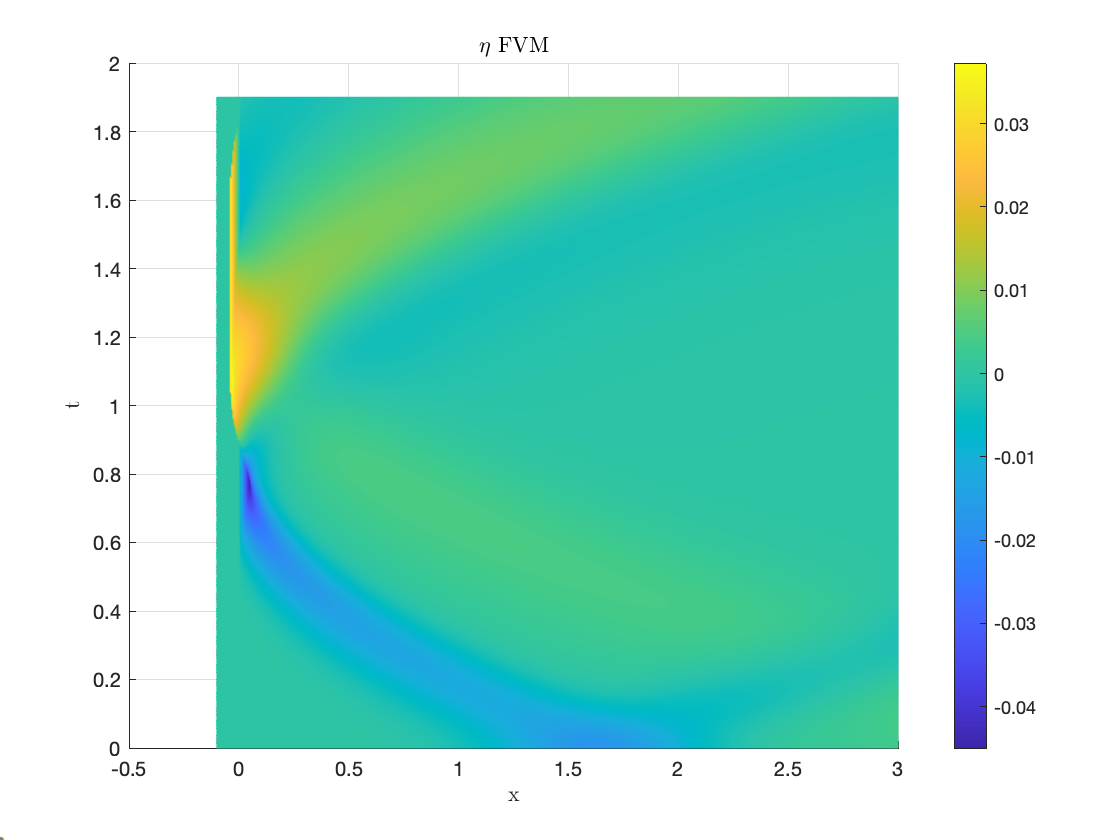
\includegraphics[scale=.25]{images/eta_FVM_0u.png} 
        \caption{Zero Velocity}
    \end{subfigure}%
    ~ 
    \begin{subfigure}[b]{0.5\textwidth}
        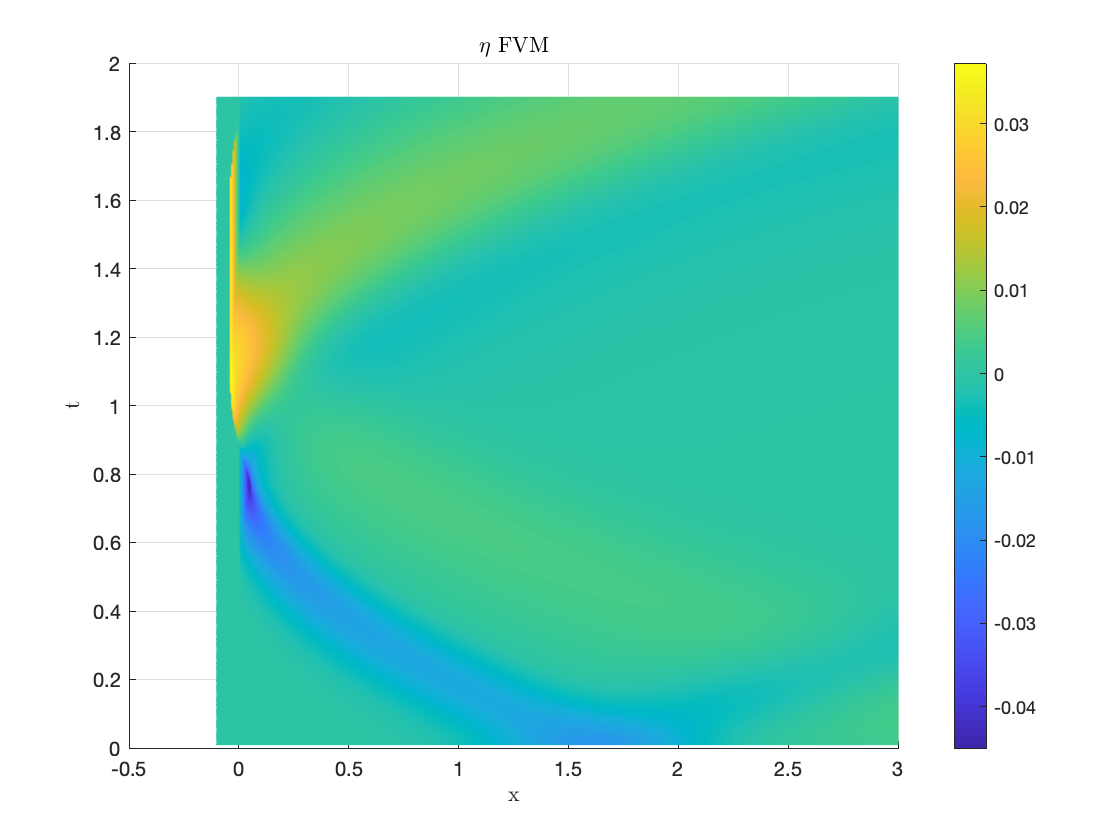
\includegraphics[scale=.25]{images/eta_FVM_non0u.png}
        \caption{Non Zero Velocity}
    \end{subfigure}
    \caption{$\eta$ FVM Solution over x:[-0.1 3] and t:[0 1.9]}
\end{figure*}


\subsection{Nicolsky 2018 Analytic}

The analytical solution of $\eta$ was computed using formulas in Nicolsky (2018). Please see Nicolsky 2018 for an extended explanation and derivation.

\[
\begin{aligned}
\psi (s, \lambda ) = \int_{0}^\infty (a(k)cos(\beta k \lambda)+b(k)sin(\beta k \lambda)) J_0(2 k \sqrt s ) dk\\
\varphi (s, \lambda ) =  s^{-1/2} \int_{0}^\infty (a(k)sin(\beta k \lambda)+b(k)cos(\beta k \lambda)) J_1(2 k \sqrt s )dk \\
\end{aligned}
\]

where

\[
\begin{aligned}
a(k) = 2k \int_{0}^\infty \psi(s_*,0) J_0(2 k \sqrt {s_*})ds_*\\
b(k) = 2k \int_{0}^\infty \varphi(s_*,0) s_*^{1/2} J_1(2 k \sqrt {s_*})ds*\\
\end{aligned}
\]

note that using change of variables $s_* = x_* + \eta_0(x_*)$  with a stipulation that $u_0 = 0$ then $a(k)$ and $b(k)$ can be transformed to

\[
\begin{aligned}
a(k) = 2k \int_{x_0}^\infty \eta_0(x_*) J_0(2 k \sqrt {x_*+\eta_0(x_*)}) (1+\eta_0^{\prime}(x) ds*\\
b(k) = 0\\
\end{aligned}
\]

This simplification was used in the zero velocity case in order to speed up computations. 
For the non-zero velocity case, the projection of $\varphi$ and $\psi$ onto $\lambda = 0$ were computed via a first order taylor expansion. Note that these equations require $\eta_0^\prime(x) > -1$.  See Nicolsky for explanation.

\[
\begin{aligned}
\Phi (s,\lambda) = \begin{pmatrix}
\varphi(s,\lambda) \\
\psi(s,\lambda)
\end{pmatrix} \\
\Phi_0(x) =  \begin{pmatrix}
u_0(x) \\
\eta_0(x) + u_0^2(x)/2
\end{pmatrix} \\
\Phi_1 = \Phi_0 + u_0(u_0^\prime A D^{-1} B \Phi_0 - B \Phi_0 - A D^{-1} \Phi_0^\prime)
\end{aligned}
\]

Chebfun was used to calculate the Hankel transform solution to the CG transform on a grid in $(s,\lambda)$ then the nonlinear Carrier Creenspan transform to $(x,t)$ Fig. 2 depicts this transform for a simple shifted Gaussian $\eta_0$. Figure 3 depicts the actual solution.


\begin{figure}
   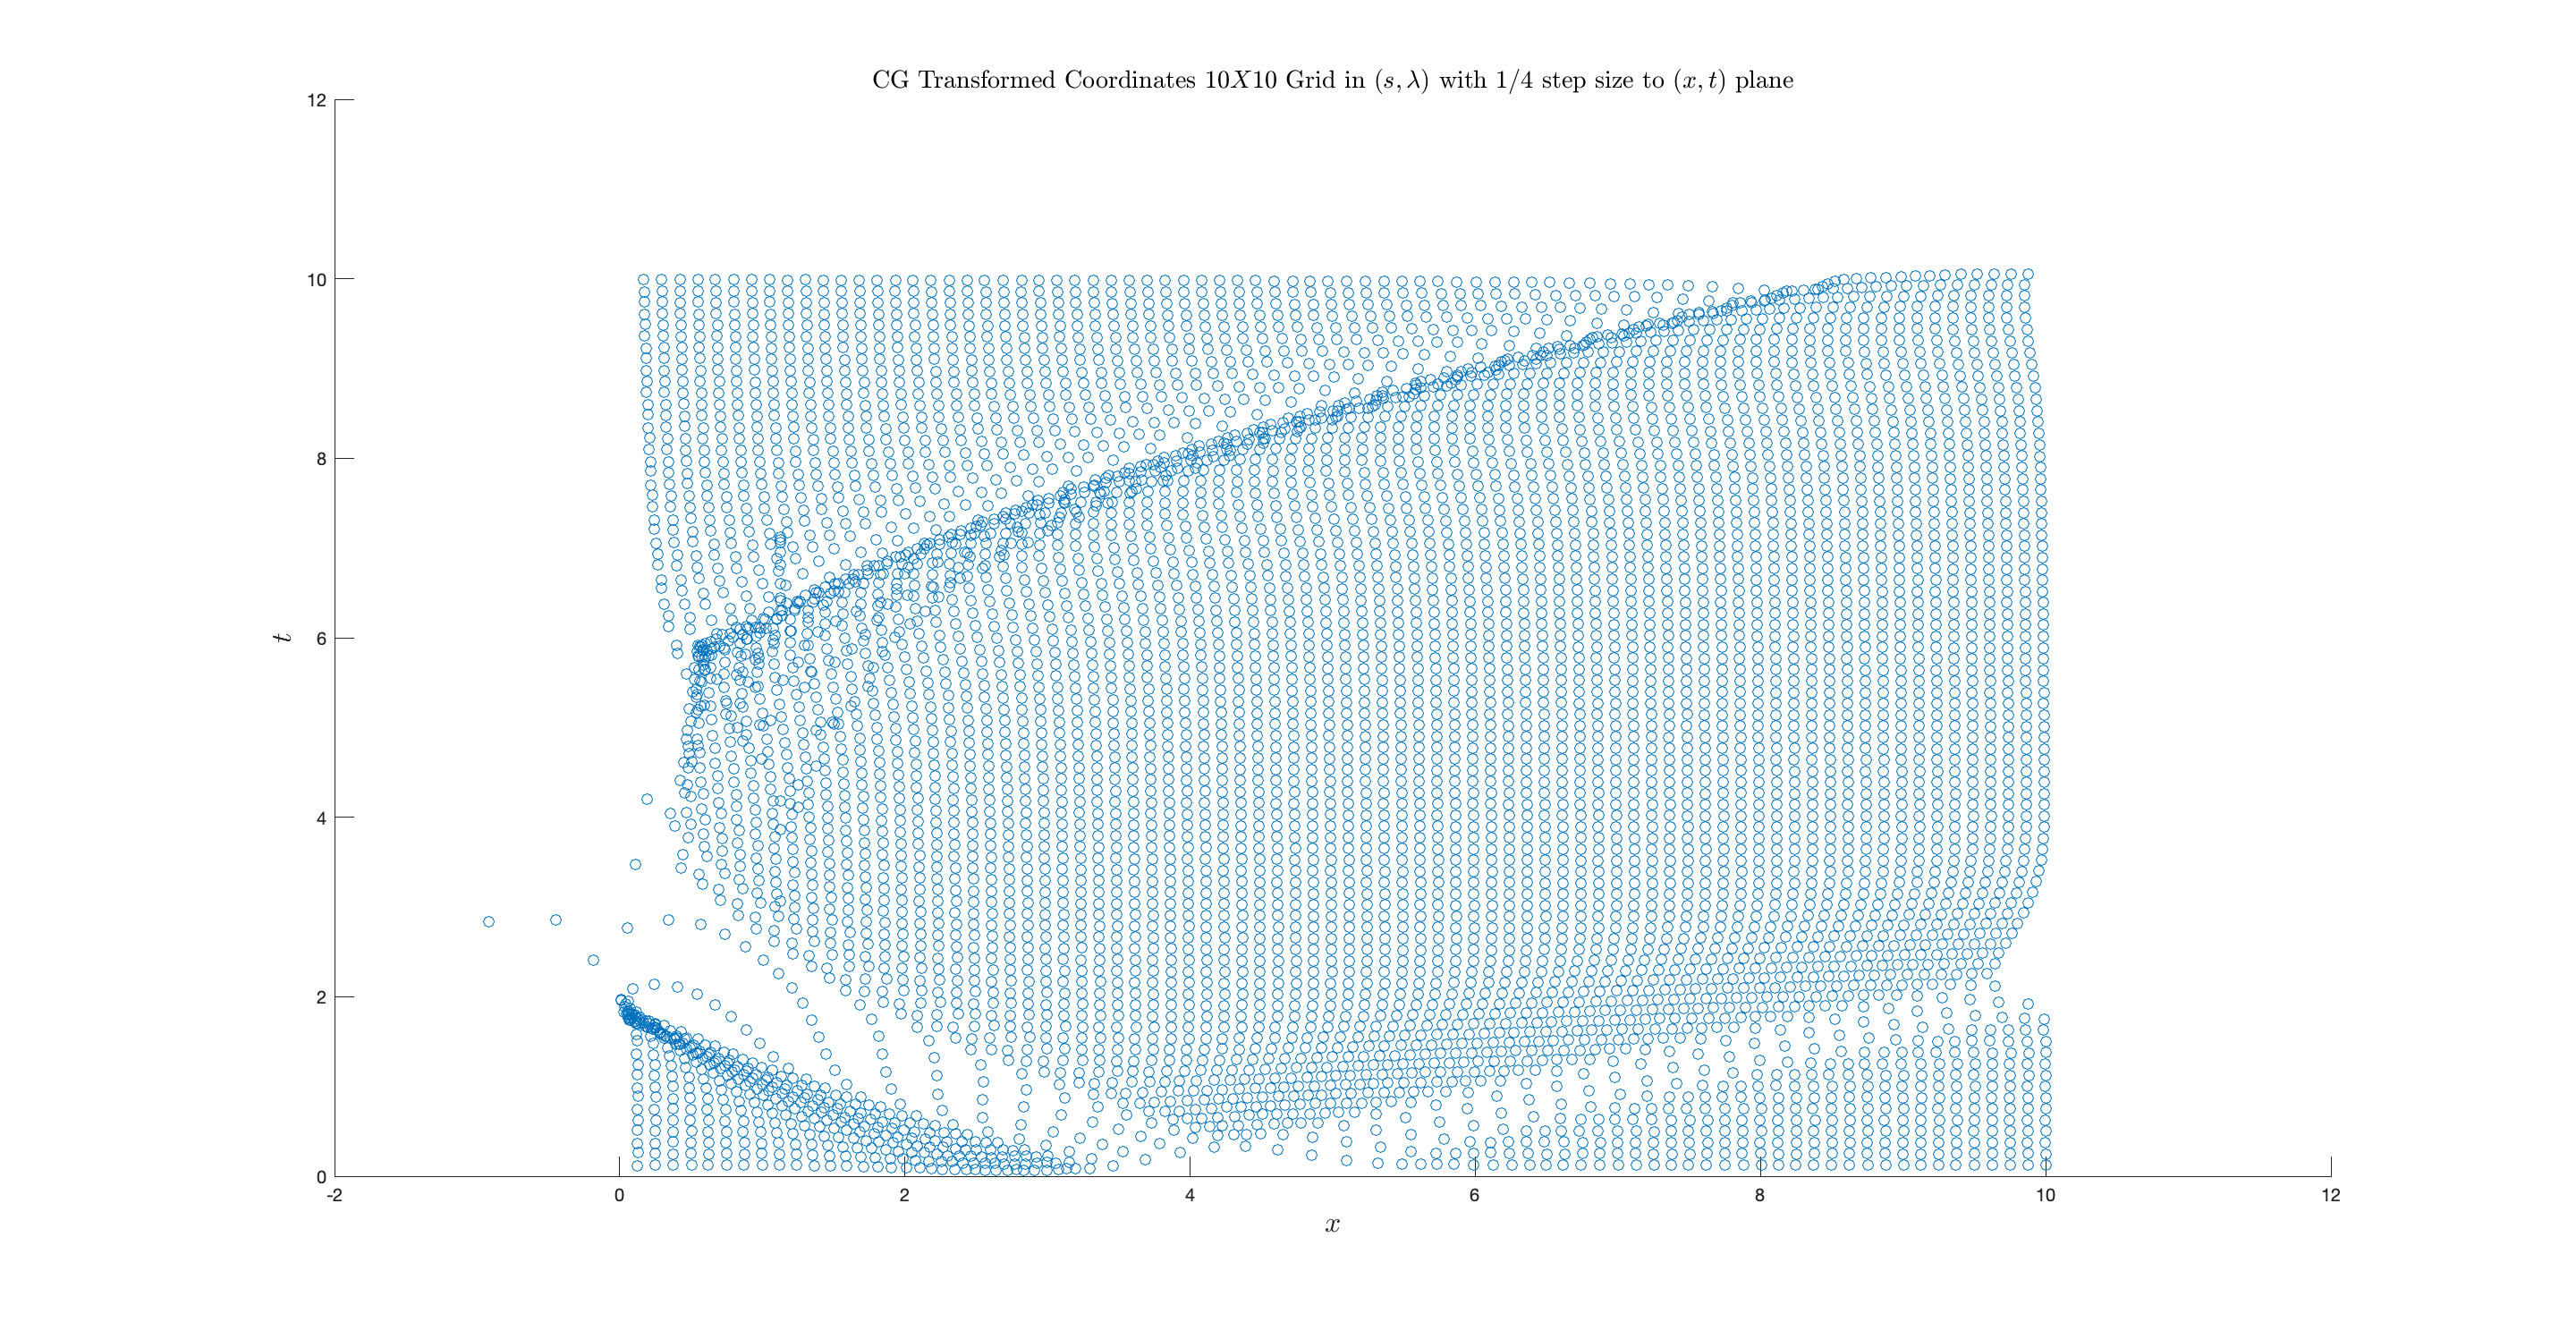
\includegraphics[scale=.13]{images/scatter.png} 
   \caption{Note the distinct non-linear nature caused by the $-u^2$ of $\eta$}
\end{figure}

\begin{figure*}[t!]
    \centering
    \begin{subfigure}[b]{0.5\textwidth}
        \centering
        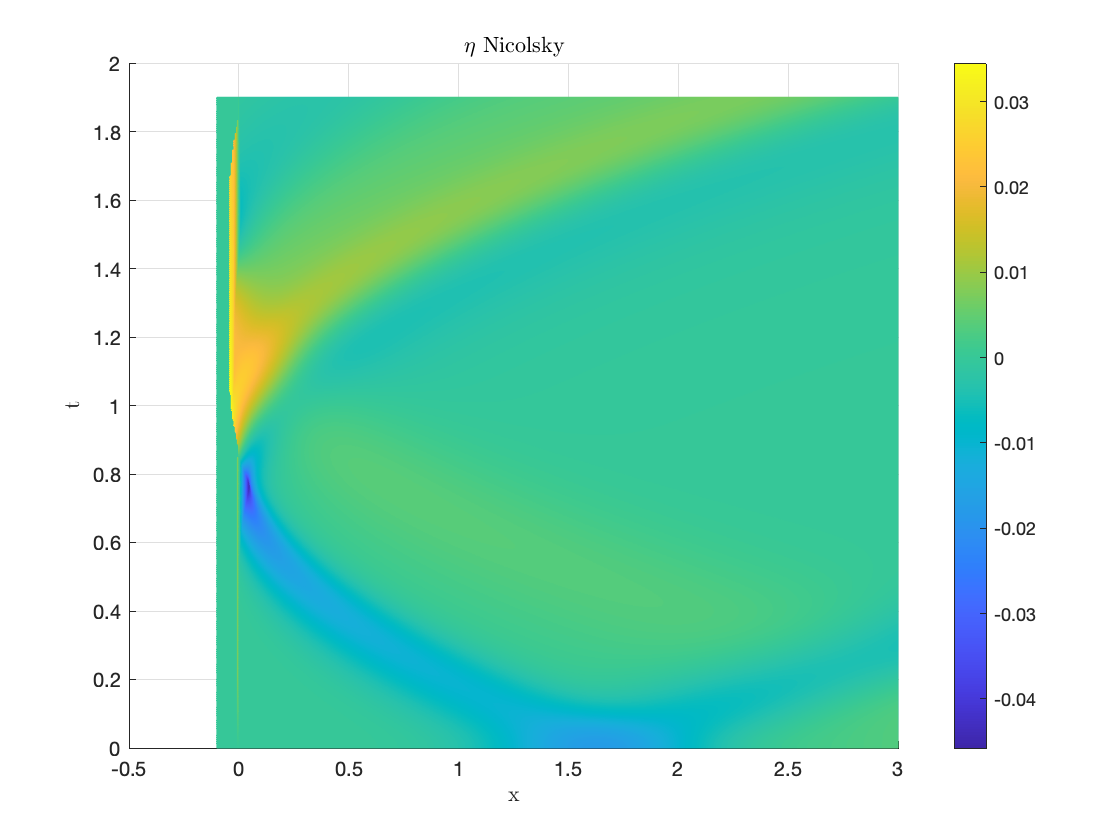
\includegraphics[scale=.25]{images/eta_Nicolsky_0u.png} 
        \caption{Zero Velocity}
    \end{subfigure}%
    ~ 
    \begin{subfigure}[b]{0.5\textwidth}
        \centering
        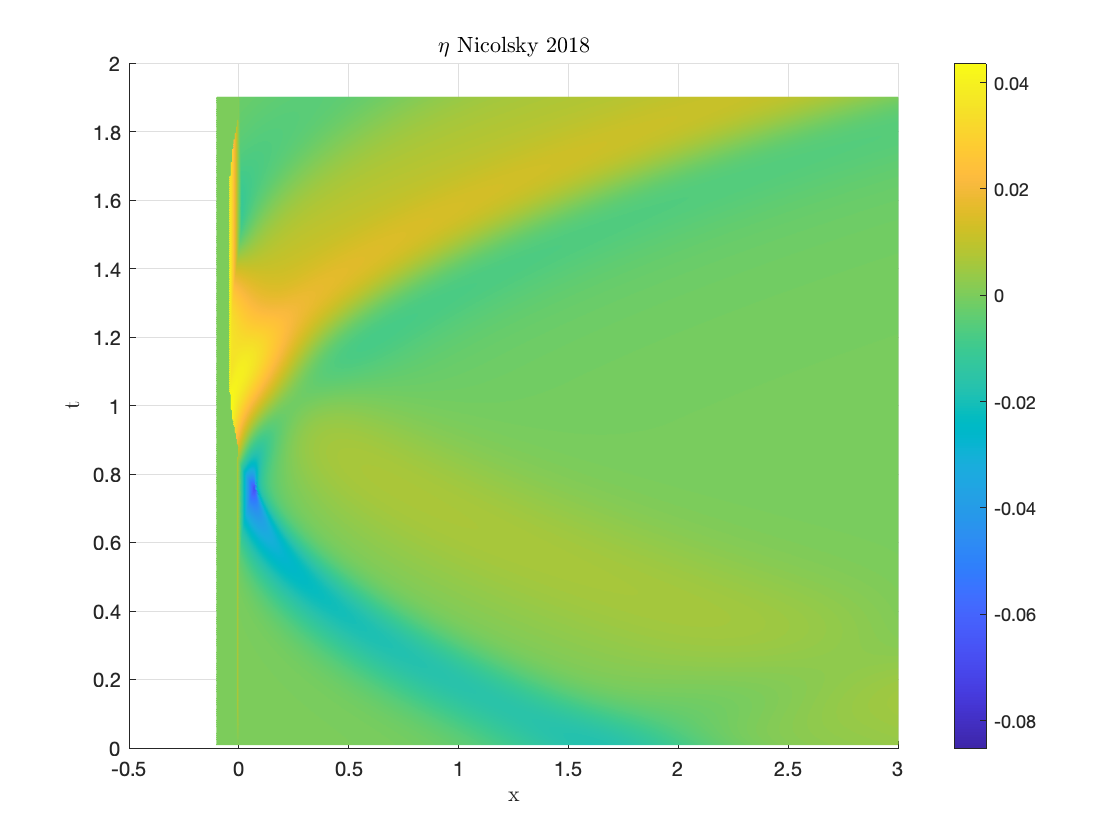
\includegraphics[scale=.25]{images/eta_Nicolsky_non0u.png}
        \caption{Non Zero Velocity}
    \end{subfigure}
    \caption{$\eta$ Nicolsky Solution over x:[-0.1 3] and t:[0 1.9]}
\end{figure*}

\subsection{Catalina 1 NOAA}

For this older analytic solution $\eta(\sigma, \lambda)$ and $u(\sigma, \lambda)$ are computed directly. However there is double integration in the computation of $\eta$ and $u$ unlike in the Nicolsky solution where single integration is used for the initial conditions and then for $\phi$ and $\psi$. Consequently, at least at this point, a highly accurate solution wasn't obtained.

$\eta_0(x)$ was transformed to $\Phi(\sigma)$ in Carrier Greenspan transformed space via

\[
\begin{aligned}
\Phi(\sigma) = -1/16 H_1 c_1 (\sigma^2 - \sigma_1^2) e^{-1/256 c_1 (\sigma^2-\sigma_1^2)^2} + 1/16 H_2 c_2 (\sigma^2 - \sigma_2^2) e^{-1/256 c_2 (\sigma^2-\sigma_2^2)^2}
\end{aligned}
\]

Then $u$ was computed via

\[
\begin{aligned}
u(\sigma, \lambda) = \int_{0}^\infty \xi^2 \Phi(\sigma) \left[ \int_{0}^\infty J_1(\omega \sigma)/\sigma J_1(\omega \xi) sin(\omega \lambda) d\omega \right] d\xi
\end{aligned}
\]

And $\eta$ was computed via

\[
\begin{aligned}
\eta(\sigma, \lambda) = -1/4 \int_{0}^\infty \xi^2 \Phi(\sigma) \left[ \int_{0}^\infty J_0(\omega \sigma) J_1(\omega \xi) cos(\omega \lambda) d\omega \right] d\xi - 1/2 u^2(\sigma, \lambda)
\end{aligned}
\]

Then $\eta(x,t)$ and $u(x,t)$ were found via an inverse Carrier Greenspan Transform. Please see NOAA for a more complete derivation. Figure 4 depicts the solution.

\begin{figure}
   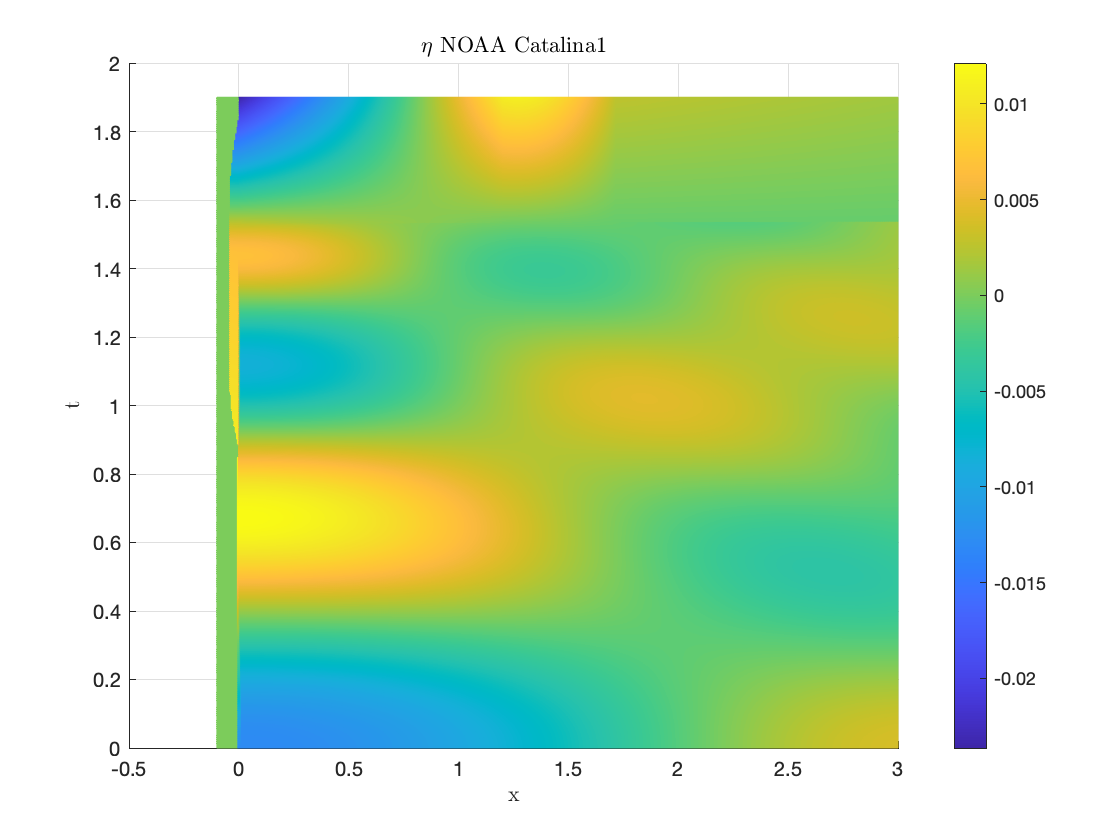
\includegraphics[scale=.3]{images/eta_NOAA_0u.png} 
   \caption{NOAA Catalina 1 Zero Velocity Solution}
\end{figure}


\section{Results}

\subsection{Zero Velocity (Catalina 1)}

Figure 5 depicts the FVM vs. Nicolsky comparison. The L2 norm is bounded below 0.055. Notice that the solution converges at $t=0$ but very rapidly diverges. One explanation for the difference is diffusion in the FVM.

\begin{figure*}[t!]
    \centering
    \begin{subfigure}[b]{0.5\textwidth}
        \centering
        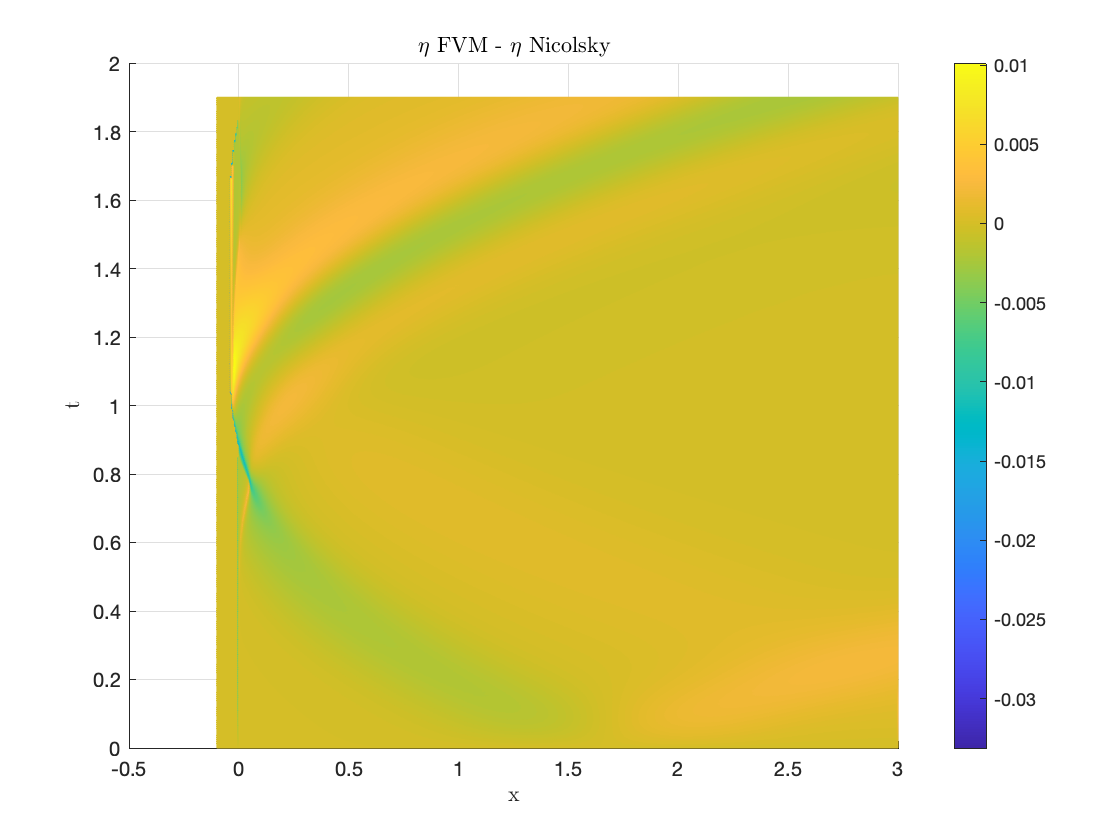
\includegraphics[scale=.25]{images/diff_FVM_Nicolsky_0u.png} 
        \caption{Difference Between FVM and Nicolsky}
    \end{subfigure}%
    ~ 
    \begin{subfigure}[b]{0.5\textwidth}
        \centering
        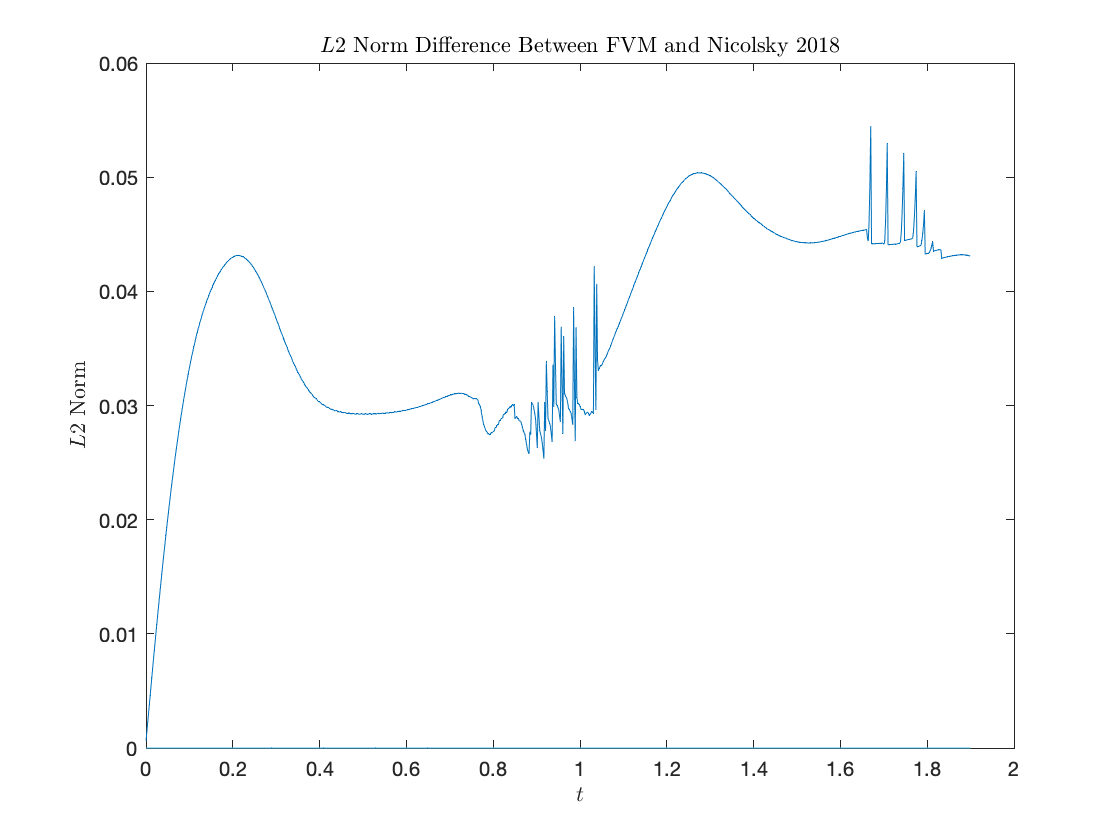
\includegraphics[scale=.25]{images/l2_FVM_Nicolsky_0u.png}
        \caption{L2 Norm at each time}
    \end{subfigure}
    \caption{$\eta$ FVM vs. Nicolsky Statistical Analysis}
\end{figure*}

Figure 6 depicts the FVM vs. NOAA comparison. The L2 norm is bounded below 0.3, which is absolutely massive. Notice that the solution doesn't converge at $t=0$ and the l2 norm remains high throughout the time interval.


\begin{figure*}[t!]
    \centering
    \begin{subfigure}[b]{0.5\textwidth}
        \centering
        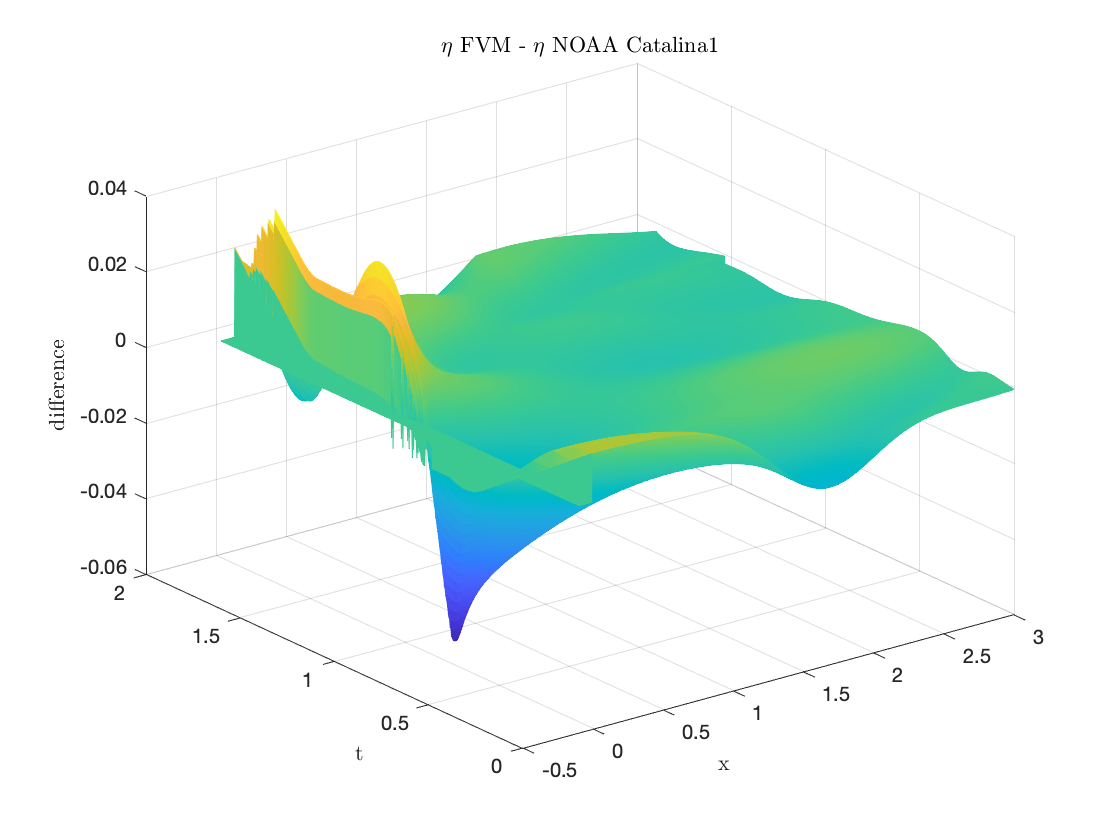
\includegraphics[scale=.25]{images/diff_FVM_NOAA_0u.png} 
        \caption{Difference Between FVM and NOAA}
    \end{subfigure}%
    ~ 
    \begin{subfigure}[b]{0.5\textwidth}
        \centering
        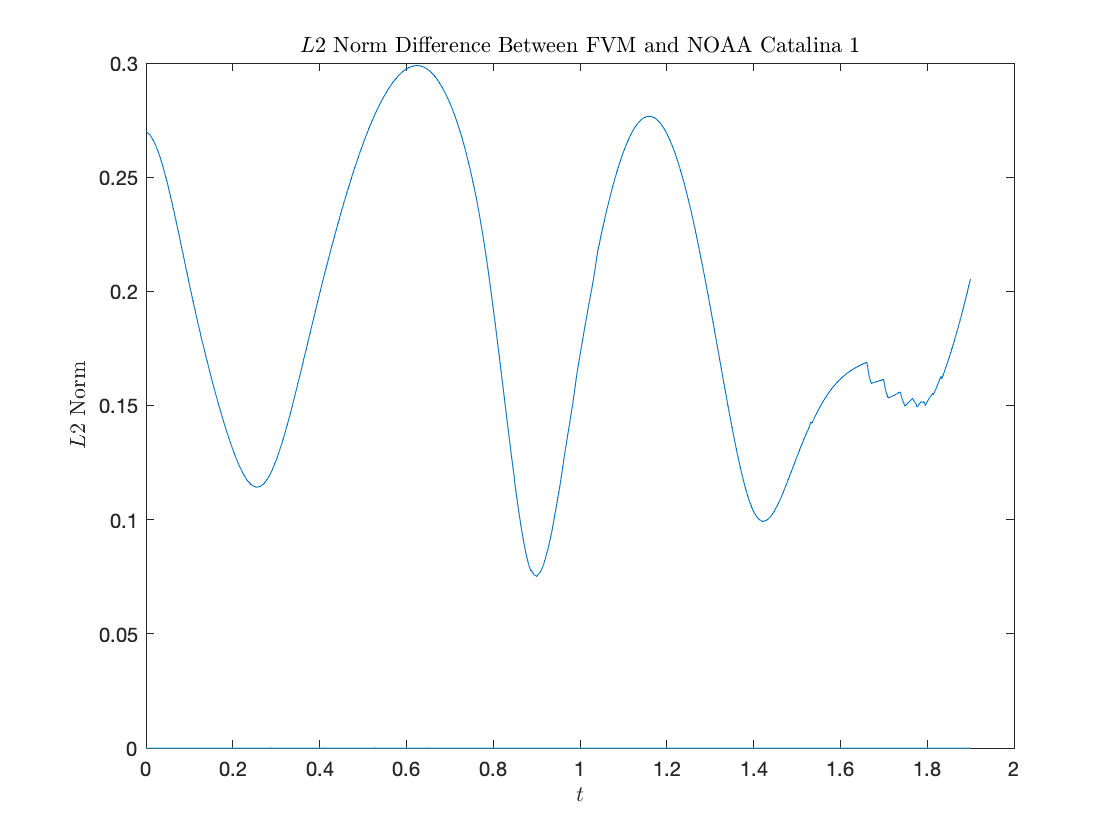
\includegraphics[scale=.25]{images/l2_FVM_NOAA_0u.png}
        \caption{L2 Norm at each time}
    \end{subfigure}
    \caption{$\eta$ FVM vs. NOAA Statistical Analysis}
\end{figure*}


\subsection{Non-Zero Velocity}

Figure 7 depicts the FVM vs. Nicolsky comparison. The L2 norm is bounded below 0.12, which is roughly double for the non-zero velocity case. Similar to the zero-velocity Nicolsky vs. FVM case, the solution converges at $t=0$.


\begin{figure*}[t!]
    \centering
    \begin{subfigure}[b]{0.5\textwidth}
        \centering
        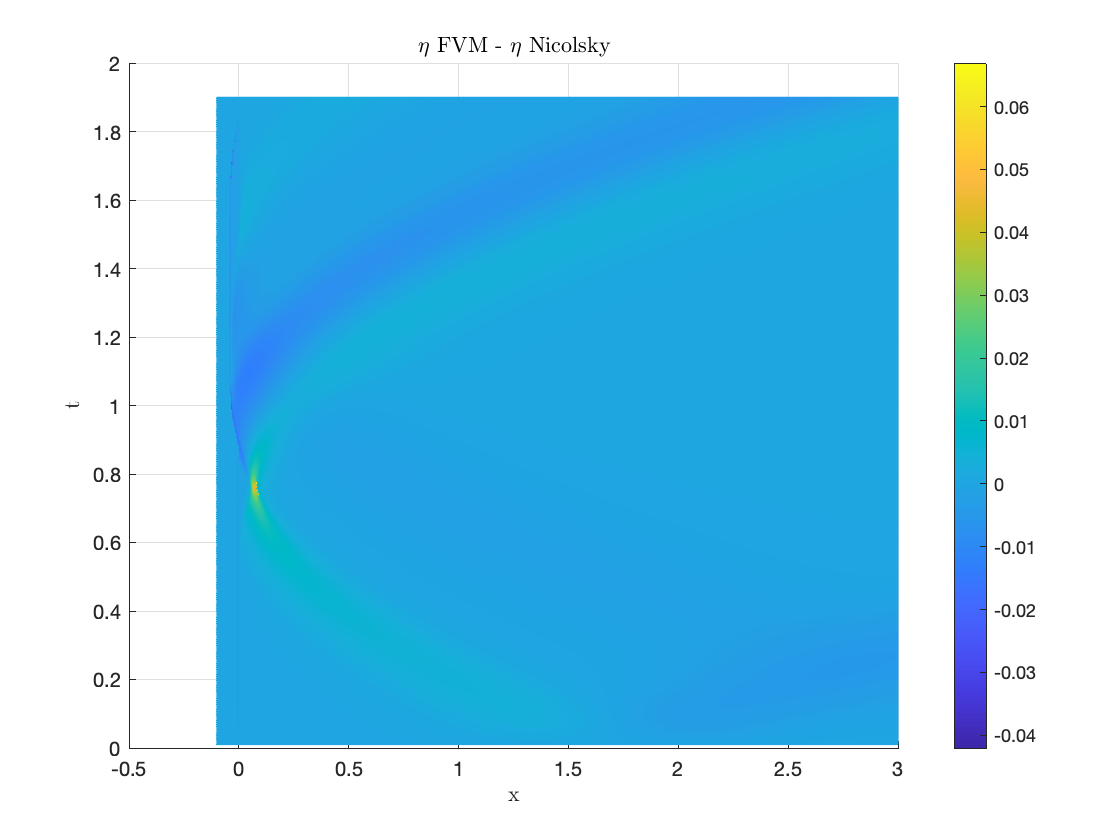
\includegraphics[scale=.25]{images/diff_FVM_Nicolsky_non0u.png} 
        \caption{Difference Between FVM and Nicolsky 2018}
    \end{subfigure}%
    ~ 
    \begin{subfigure}[b]{0.5\textwidth}
        \centering
        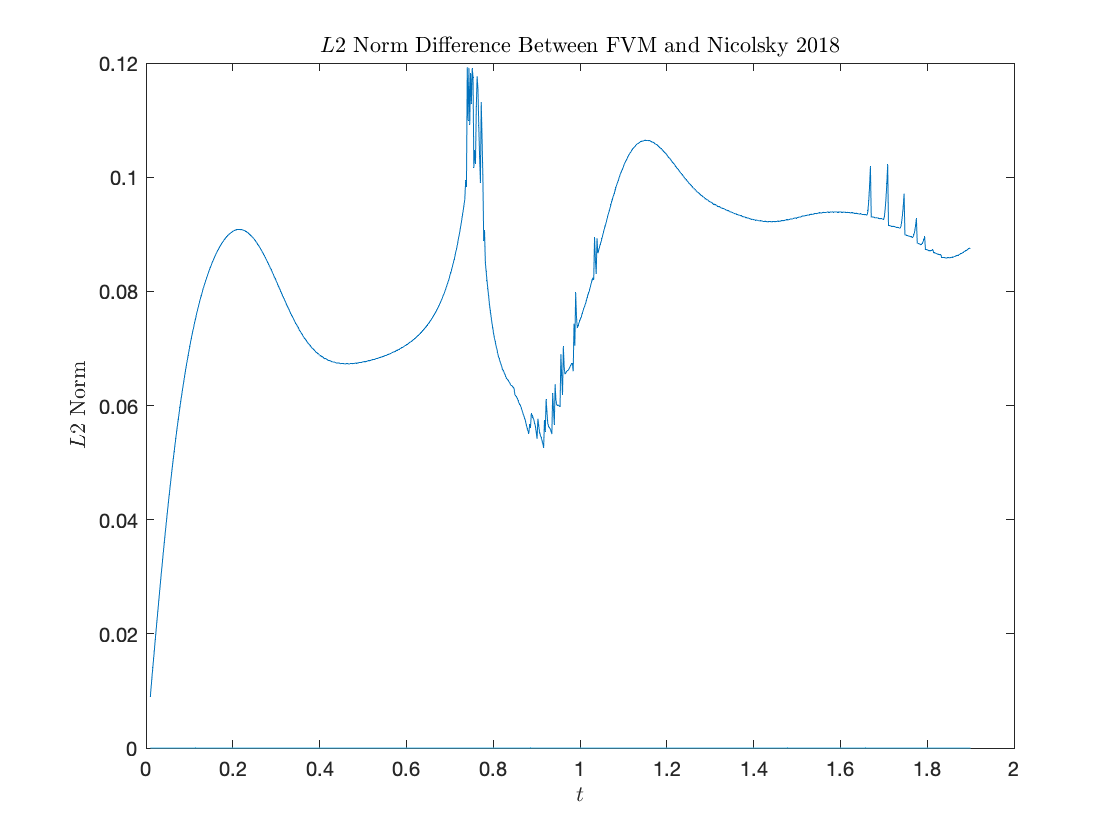
\includegraphics[scale=.25]{images/l2_FVM_Nicolsky_non0u.png}
        \caption{L2 Norm at each time}
    \end{subfigure}
    \caption{$\eta$ FVM vs. Nicolsky Non Zero Velocity Statistical Analysis}
\end{figure*}


\end{document}
